
\section{HPX} \label{sec:hpx}
HPX is a C++ library and runtime system for task-based parallellization. It treats both intra- and inter-node parallelization within an homogeneus interface and it adheres to the C++11/14 standard, which introduced basic support for task-based parallelism.

It features a global address space, the ability to migrate work remotely in the proximity of data, and it supports task dependencies and continuations.
Its task scheduler is designed to introduce minimal overhead and supports very fine-grained tasks down to \textasciitilde$1\mu s$\cite{grubel2016using} and work-stealing for automatic load balancing.
It also delivers a powerful performance monitoring system which allows a program to query various performance metrics at runtime and to react accordingly.

\subsection{The ParalleX execution model}\label{subs:parallexModel}
HPX implements the ParalleX \cite{kaiser2009parallex} execution model, which leverages medium- and fine-grained task parallelism and aims at optimizing both parallel efficiency and programmability of parallel code.

The key highlights of this model are:
\begin{description}
	\item [Asynchronous task execution] Functions are meant to be called asynchronously and to yield a proxy for the actual return value. Such a proxy is called a \emph{future} (figure \ref{fig:futureFlowDiagram}). The program will need to synchronize only when the actual return value is needed, e.g. for a later computation. If the task was able to complete between the asynchronous call and the synchronization step, then no waiting time is needed.
	\begin{figure}[t]
	 	\begin{center}
	 		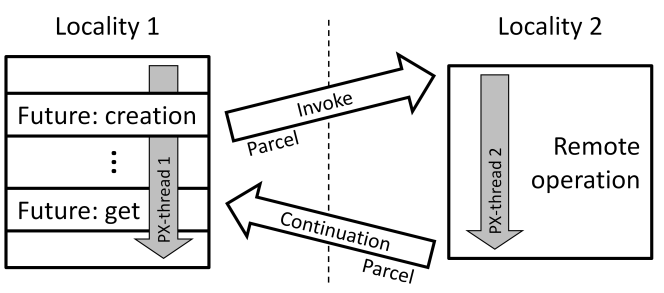
\includegraphics[scale=0.3]{Figures/futureFlowDiagram.png}
	 		\caption{Schematic flow diagram of a future\cite{kaiser2009parallex}.}\label{fig:futureFlowDiagram}
	 	\end{center}
	\end{figure}
	\item [Lightweight synchronization] Not only we can use futures but we can also make an asynchronous call depend on one or several futures: this enables the runtime system to keep track of the actual dependencies and removes the need for expensive synchronization mechanisms, such as global barriers.
	\item [Active Global Address Space (AGAS)] ParalleX features a global address space abstraction service. This address space spans all the available hardware entities, called \emph{localities}.
	The peculiarity of AGAS is that it is not a \emph{partitioned} global address space (PGAS): in PGAS the global address space is statically partitioned across the available localities and moving an object to a different locality requires a change of its address; in AGAS the address space is dynamically and adaptively mapped to the underlying localities, allowing transparent migration of objects across localities while they can still retain their \emph{global identifier (GID)}.
	\item [Message-driven queue-based scheduling] When a task execution is requested, which may be on any remote locality, an active message, called \emph{parcel}, is sent to the target locality. This triggers the creation of a \emph{PX-Thread}\footnote{From now on PX-Threads will be referred to just as \emph{threads}.}, which will be queued and then scheduled for execution on the OS thread(s) managed by the target locality. This form of message passing is therefore not limited to data and it does not require explicit receive operations to be invoked on the target side. The queuing and scheduling is designed in a way to allow for idling processors or cores to \emph{steal} work from the queues of other ones: this allows for efficient load balancing and prevents starvation\todo{maybe explain starvation}.
\end{description}

% This clearly differentiates from the usual \emph{Single Program Multiple Data (SPMD)} approach used in MPI and OpenMP, as there is no need to explicitly take care 

\subsection{HPX high-level architecture}
HPX implements the ParalleX model as a C++ library adhering to C++11/14 standard interfaces for task-based parallelism.
It aims to address the four main factors that prevent scaling in scaling-impaired applications, which are referred to as \emph{SLOW}\cite{kaiser2014hpx}:
\begin{description}
	\item [Starvation] Not all resources are fully utilized because of a lack of enough concurrent work to execute.
	\item [Latencies] Intrinsic delays in accessing remote resources.
	\item [Overheads] The overheads of parallelization, i.e. the work required for management of the parallel computation and any extra work which would not be necessary in a sequential version.
	\item [Waiting for contention resolution] Any delay caused by oversubscription of shared resources.
\end{description}

HPX tries to deal with the above problems by embracing the following design principles: focus on latency hiding instead of latency avoidance, embrace fine-grained parallelism, leverage constraint based synchronization, use adaptive locality control instead of static data distribution, move work to data instead of data to work and embrace message driven computation instead of message passing.\cite{kaiser2014hpx}

[\TODO we must add something more here...]

The high-level fundamental components of HPX are:

\begin{figure}[b]
 	\begin{center}
 		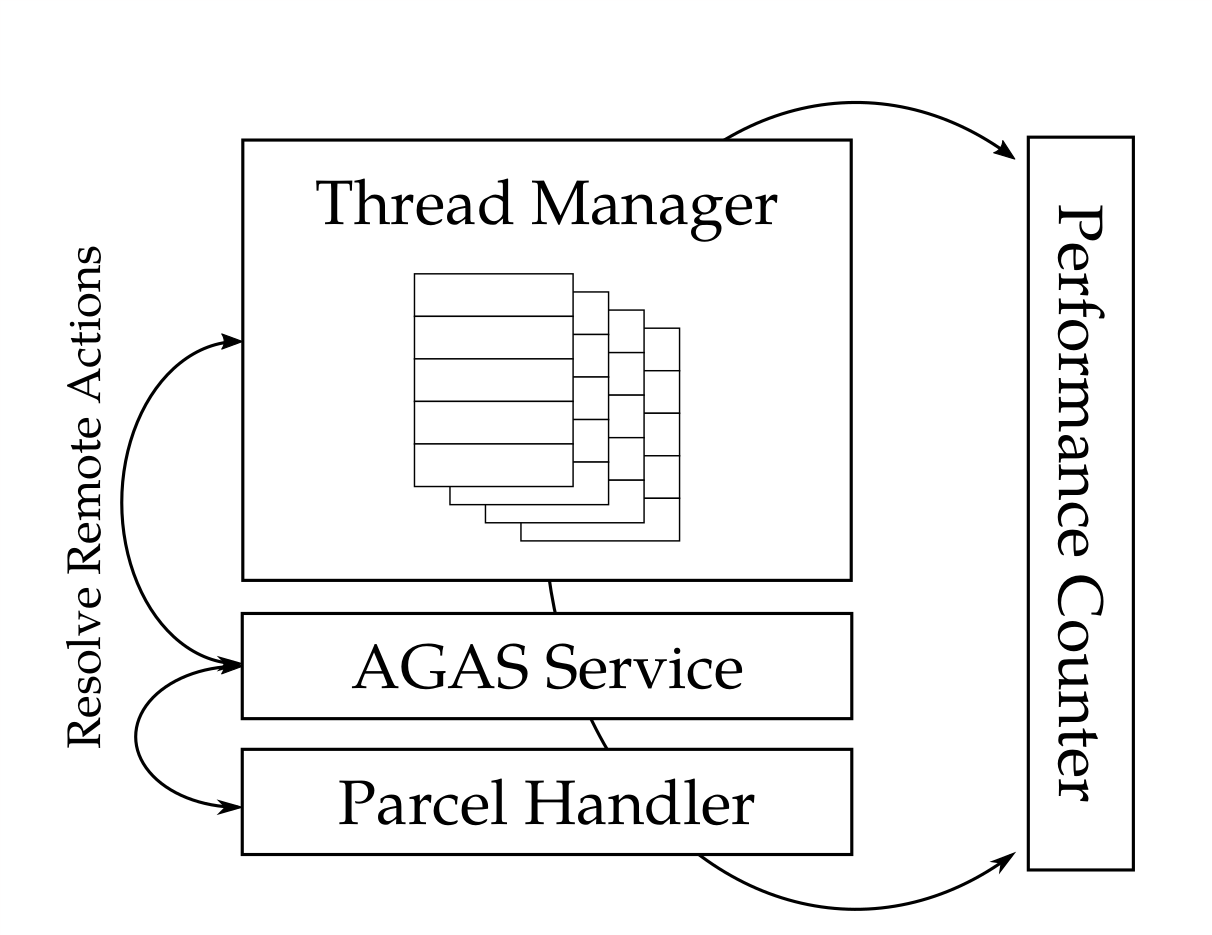
\includegraphics[scale=0.18]{Figures/hpxArchitecture.png}
 		\caption{Overview of the HPX runtime system components\cite{heller2017hpx}.}\label{fig:hpxArchitecture}
 	\end{center}
\end{figure}
\\ 

\paragraph{Threads \& Scheduler}
When a new thread is created, HPX queues it at an appropriate locality and it then schedules it according to configurable policies. The scheduling is cooperative, i.e. non-preemptive, since preemption and the overhead associated to content switches would not make sense in the context of a single application. Threads are scheduled onto a pool of OS threads, which are usually one per core, whitout requiring any kernel transition and thus removing all the overhead associated to the creation of OS threads.
\\ 

\paragraph{Parcels}
Parcels are the HPX implementation of active messages, i.e. messages which can not only deliver data but also trigger execution of methods on remote localities.
Parcels carry the GID of the destination, a remote action, arguments for the action (data) and, if required, a continuation.
\\ 

\paragraph{Local Control Objects}
``Local Control Objects (LCOs) control parallelization and synchronization of
HPX applications. An LCO is any object that may create, activate, or reactivate
an HPX thread.''\cite{grubel2016dynamic}

The most prominent LCOs delivered by HPX are \emph{futures} and \emph{dataflow} objects. Futures are proxies for values which might not have been computed yet and include a synchronization when the actual value is requested. Dataflow objects are instead LCOs which depend on a set of futures as input and they return themselves a future for the result of their continuation.

Futures and dataflow LCOs allow to express the true data dependencies within an application and to translate them into the associated execution tree and necessary synchronizations.
\\ 

\paragraph{Active Global Address Space}
As already mentioned in \ref{subs:parallexModel}, one of ParalleX main features is the AGAS: HPX implements an AGAS service which delivers those functionalities.
\\ 

\paragraph{Performance monitoring system}
HPX implements a performance monitoring system based on a variety of \emph{performance counters}, which are objects providing metrics and statistics on the performance of
\begin{enumerate*}[label={(\roman*)}]
	\item hardware,
	\item application,
	\item HPX runtime and
	\item OS
\end{enumerate*}.
Performance counters are first class objects, they are therefore addressable by their GID from any locality and are available to both the application and the HPX runtime for performing introspection at runtime on how well the system is performing.\cite{kaiser2014hpx}
Performance counters expose a predefined interface and HPX exposes specific API functions allowing to create, manage and release counters, as well as to read their data in a structured way.
Performance counters are not only available from within the application. By passing standard command line flags to an HPX application we can conveniently have the performance counters of interest periodically logged to screen or to a file during execution. Performance counter can also be accessed in realtime by other utilities by connecting to a running HPX application through its parcel transport layer\cite{kaiser2014hpx}.
They are useful tools for performance analysis and for identifying bottlenecks, and they are even more useful as they provide the necessary infrastructure for building resource awareness into an HPX application\cite{grubel2016using}.


\section{Resource awareness in HPX} \label{sec:hpxRAC}
HPX supports resource awareness by design and, up to a certain degree, automatically.
Its execution model is based on the assumption that threading, synchronization and data distribution must not be exposed to the programmer and must be handled automatically behind the scenes. HPX provides an abstraction for parallelism which does not require the programmer to think about localities, send/receive instructions, threads or barriers, which are referred to by Hartmut Kaiser, the HPX project lead, as the ``GOTOs of parallel computing''\cite{kaiser2014goto}. HPX also encourages the programmer to define fine grained tasks, while the runtime takes care of the actual scheduling and synchronization. This has the positive side effect of making the runtime adaptive, by default, in terms of load balancing.

No comprehensive analysis of resource awareness in HPX has been performed so far, therefore I below report what I believe to be the main features of HPX that can support resource awareness.
\\ 

\paragraph{Task scheduling}
The HPX thread manager and the way it schedules queues for each worker thread are configurable with three main pre-defined policies\cite{heller2017hpx,amatya2014parallel}:
\begin{description}
	\item [Static] The thread manager maintains a work queue for each worker thread and tasks are distributed to queues in a round robin fashion. In this policy there is no way for tasks to change their allocation to queues.
	\item [Local] This is the default scheduling policy. In this policy the thread manager maintains a work queue for each worker thread plus extra special queues for high and low priority tasks. Work is distributed to queues as in the static policy, but as soon as a load imbalance is detected on the worker threads, work is stolen from higher loaded threads and distributed to lower loaded ones.
	\item [Hierarchical] In this policy the thread manager maintains a tree of work queues where the leaves correspond to the worker threads. New tasks are always enqueued at the root of the tree and then trickle down the hierarchy. In this policy work can be stolen at any level of the tree, from queues belonging to the same level.
\end{description}

From the above policies we can see one very important behaviour of the task scheduler which allows for resource awareness when enabled: \emph{work stealing}.

As mentioned, work stealing occurs as soon as a load imbalance is detected among different worker threads' queues.
This is optionally done in a NUMA-aware way, i.e. the work is redistributed preferentially within the same NUMA domain in order to preserve memory access performance.

Work stealing therefore operates an automatic load balancing action at runtime and is therefore a means to get adaptivity out of the box with HPX.

An important factor that has to be taken into account for effective task scheduling is data --- both temporal and spatial --- locality. Performing task scheduling blind to data locality can lead to substantial performance degradation \cite{connelly1994workload}, while locality aware scheduling can effectively reduce the number of data load and transfer operations and their associated overhead.

HPX can include data locality awareness in task scheduling and its task dependency semantics allows hierarchical grouping of tasks, therefore naturally exposing different levels of data locality \cite{amatya2014parallel}.

Furthermore, as shown by Grubel \cite{grubel2016dynamic}, the HPX task scheduler can be extended to consume performance counters to achieve automatic tuning of task grain size. This kind of feedback loop allows the task scheduler to react to real-time performance metrics such as scheduling overheads and task execution time to dynamically adapt its behaviour to achieve better performance.
\\ 

\paragraph{AGAS}
Although AGAS does not a priori imply resource awareness, I believe it is an important feature within HPX in support for adaptivity. It ``is a dynamic and adaptive address space
which evolves over the lifetime of an application'' and ``is the foundation for dynamic locality control as objects can be moved to other localities without changing their global address''.\cite{kaiser2014hpx}
This allows implementing mechanisms to relocate objects to different localities in response to performance metrics and resource constraints \cite{amatya2014parallel} and still being able to access them from the rest of the application in a transparent way. The migration decision has to be based on performance metrics and be aware of resources also for what concerns the target locality, in order to ensure a better performance as outcome. This requires a performance monitoring infrastructure allowing access to metrics for remote localities, which in HPX is fullfilled by performance counters.
The object relocation logic can be therefore completely decoupled from the code accessing the objects and this clearly allows a much cleaner and modular code and it fullfills the underlying design goal of having parallelization and data distribution internalities as much hidden from the programmer as possible.
\\ 

\paragraph{Percolation}
Percolation is a special use of parcels which allows directly targeting hardware resources, instead of logical data data objects, as destination.
Percolation provides therefore a way to address specialized hardware --- such as gpGPUs and FPGAs --- directly through the parcel layer, enabling to provide work to these accelerators as well as getting back the results in a clean way.
The percolation mechanism in HPX is aware of the characteristics of specialized hardware resources and can therefore route relevant tasks to these resources in a efficient way \cite{amatya2014parallel}.
\\ 

\paragraph{Performance counters}
Performance counters are a central feature of HPX and play a key role in its resource awareness capabilities.

An efficient performance measurement framework is a requirement for any runtime system targeting fine grained parallelism and exascale computing: it needs to be able to gather and manage a massive amount of information, while at the same time being as unobtrusive as possible, in order to minimize its perturbations to the application performance. Furthermore, such a measurement framework needs to be able to scale as required by applications and available resources \cite{amatya2014parallel}.

Traditionally performance measurements are used for post-run analysis, for either debugging or optimization of parameters.
However as the degree of parallelism increases --- and so do performance-affecting parameters --- it becomes more and more crucial to have well-integrated dynamic performance measurement capabilities and to leverage the measured data for dynamic tuning of application parameters.

[\TODO refer to \cite{grubel2016using}]

%eof
